\chapter{Single-atom resolved momentum measurement of lattice Bose gas}

\label{sec:chapter_3}

blah blah blah

\section{Metastable Helium}

Metastable Helium, noted $\mathrm{He}^*$, is kind of an odd atom in the ensemble of species that we know how to bring to quantum degeneracy. Its most important feature, which is actually the reason why we chose this atom to measure correlation functions in momentum space, is the existence of the metastable state $2 \ ^3 S_1$. This excited state is called metastable for its very long lifetime of the order of $8,000 \ \mathrm{s}$, far larger than what is required for experiments. Very interestingly, as Helium is a noble gas, the amount of energy required to excite Helium into its metastable state is quite large, $19.8 \ \rm{eV}$. This large energy is sufficient for a metastable Helium atom to extract an electron from an electronic surface. This opens the way for \textbf{electronic detection} techniques, in opposition to the much more widely spread optical detection techniques, that allows for \textbf{single atom detection} as we will see in this chapter. In addition, the energy level structure (see Fig.-\ref{fig:niveaux}) is well adapted to laser cooling with a transition in the near-infrared around $\lambda_0 \simeq 1083 \ \mathrm{nm}$ for which reliable laser sources are available. Metastable Helium was actually amongst the first atoms to be brought to quantum degeneracy with the first BEC of $\He$ being obtained in 2001 simultaneously at the Institut d'Optique and Laboratoire Kastler Brossel in France. Helium also has the advantage to have a stable, albeit very rare and expensive fermionic isotope $^3 \He$ that has also been brought to quantum degeneracy at the Amsterdam LaserLab in 2006.

In spite of all these advantages, $\He$ comes with a few experimental difficulties that explain why they are actually quite few $\He$ experiments over the world. First, Helium is a very light atom and this comes with some very practical difficulties like the need for pre-cooling with liquid nitrogen and quite long Zeeman slowers. Second, $\He$ is subject to Penning collisions that bring back an atom to the ground state to ionize the other:

\begin{equation}
    \He + \He \rightarrow \mathrm{He} + \mathrm{He}^+ + \mathrm{e}^{-}
\end{equation}

Such a reaction thus results in the loss of two atoms and must be avoided. \NOTE{FINIR}

\begin{figure}
    \centering
    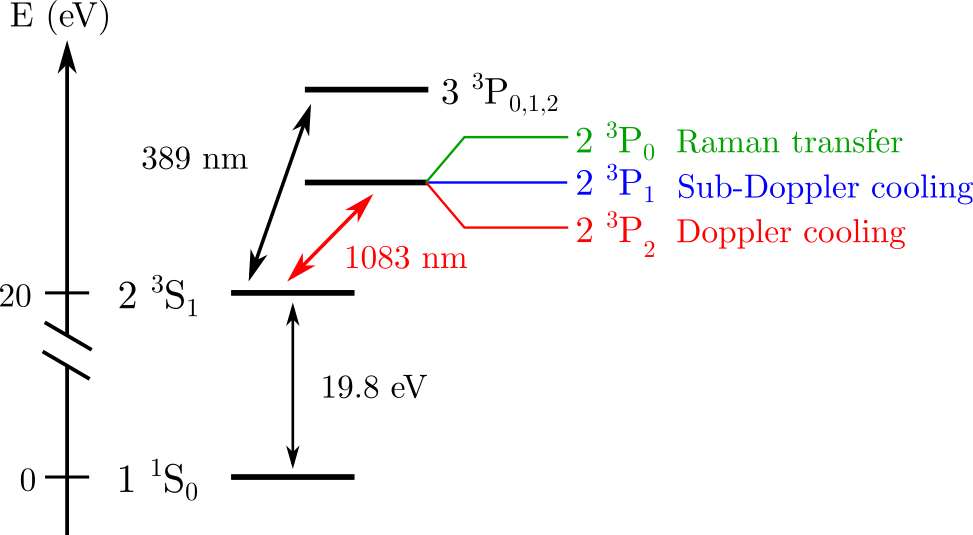
\includegraphics[width=0.9\textwidth]{Fig/Chapter3/niveaux.png}
    \caption{Energy levels of the Helium atom. The metastable state is the triplet state $2 \ ^3S_1$ that we will call the ground state of the metastable Helium atom. Laser cooling is performed on the optical transition $2 \ ^3S_1 \rightarrow 2 \ ^3 P$ of wavelength $\lambda_0 \simeq 1083 \ \mathrm{nm}$. More specifically, we address the transition to  $2 \ ^3 P_2$ or $2 \ ^3 P_1$ depending on the cooling scheme (respectively Doppler and sub-Doppler), as well as the transition to  $2 \ ^3 P_0$ to perform two-photon Raman transfer as we will detail later on.}
    \label{fig:niveaux}
\end{figure}

In the following, we will detail the different experimental steps used to bring a gas of metastable Helium to quantum degeneracy.

\section{Bose-Einstein Condensation of metastable helium}

\subsection{The source}

To begin the experimental sequence, we first need to excite helium atoms in the metastable state. As the energy difference between the ground-state and the metastable state is very large, it is impossible to excite the atoms optically, we therefore rather do it through a plasma discharge. The setup is illustrated on Fig.-\ref{fig:source}. The plasma forms between a metallic needle connected to a high voltage power supply ($\sim 2.8 \ \mathrm{kV}$) and the grounded skimmer. The needle is held in a glass tube that is glued to a \textbf{Boron-Nitride (BN)} piece, in which a small hole is pierced for atoms to flow through. The piece is inserted into a larger copper piece cryogenically cooled with liquid nitrogen. The role of the Boron-Nitride piece is two fold. First, the good thermal properties of the Boron-Nitride allows the piece to be cooled via the contact with the copper, cooling down in turn the atoms. This is necessary to preliminary reduce the speed of the atoms before laser cooling as we will discuss in the next paragraph. Second, the piece isolates the high voltage needle from the grounded copper to avoid plasma formation in unwanted places.

\begin{figure}
    \centering
    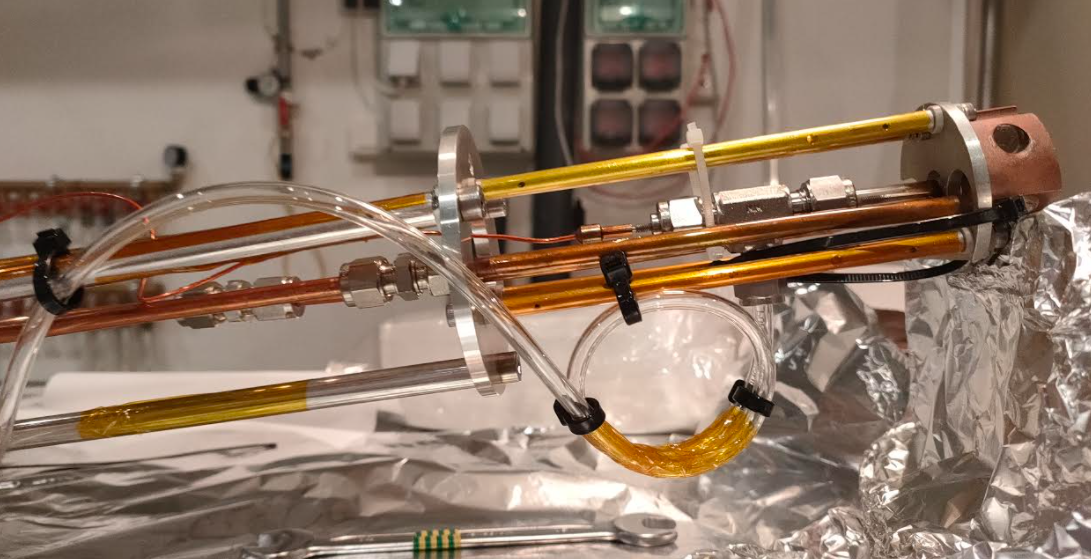
\includegraphics[width=0.9\textwidth]{Fig/Chapter3/source.png}
    \caption{Metastable helium source. a) Illustrative drawing of the source apparatus. Helium atoms (blue arrows) are sent into a glass tube glued into a pierced boron-nitride (BN) piece. A plasma forms between the high voltage needle and the grounded skimmer, exciting the atoms in the metastable state (red arrows). The boron nitride is cooled by thermal contact with a copper (Cu) piece in which liquid nitrogen flows, allowing to significantly reduce the speed of the atoms. b) Photograph of the source apparatus. The red square illustrates what is represented on the drawing.}
    \label{fig:source}
\end{figure}

The source is a quite sensitive part of the experimental apparatus and was often subject to problems during the span of this thesis. Here are a few things that we learned through the different repairs:

\begin{itemize}
    \item The needle has the tendency to deteriorate over time. When this happens, some metallic particles fall from the needle and end up clogging the small hole in Boron-Nitride, preventing the atoms to flow through. We replaced the needle with a standard metallic cylinder, hoping that it would not deteriorate as fast. While we still could form the plasma without the needle shape, the cylinder still deteriorates, requiring regular operations every few months to unclog the Boron-Nitride piece.
    \item The diameter of the Boron-Nitride piece needs to be very well adapted to the inner diameter of the copper piece to ensure a good thermal contact and to prevent the Boron-Nitride from moving when temperature changes.
    \item The glue can contract at low temperatures and add mechanical constraints on the glass tube, sometimes breaking it and causing unwanted atom leakage.
\end{itemize}

Let us now move on the next experimental step, laser cooling.


\subsection{Laser cooling}

Our experimental cooling sequence revolves around two types of laser cooling: Doppler and sub-Doppler cooling. Doppler cooling revolves around the absorption of resonant, counter-propagating photons by a two-level atom, reducing its momentum. The absorbed photons are re-emitted spontaneously in a random direction of space, meaning that after a large number of absorption/emission cycles, the variation of momentum induced by spontaneous emission averages out. The only contribution is thus the one of absorption contributing to slow the atom down. This effect is called Doppler cooling as the frequency of the photons seen by the atoms changes with their speed because of the well-known Doppler effect. It is then necessary to account for the Doppler effect to ensure that the photons are resonant with the two-level transition of interest to ensure proper cooling. On the other hand, sub-Doppler cooling designs a variety of cooling techniques revolving around multi-level atomic structures. These techniques allow to reach lower temperature than Doppler cooling, at the expense of small velocity captures, attainable with prior Doppler cooling. 

As shown on Fig.-\ref{fig:niveaux}, we use the $2 \ ^3 S_1 \rightarrow 2 \ ^3 P_2$ transition for Doppler cooling. The state $2 \ ^3 S_1$ has three sub-states $m_j=\{-1,0,+1\}$ whereas the state $2 \ ^3 P_2$ has 5 $m_j=\{-2,-1,0,+1,+2\}$. By using circularly polarised light allowing transitions that increase or decrease $m_j$ by $1$, the transition between these two-states can be assimilated as an effective two-level transition after a few cycles of absorption/emissions, making it well suited for Doppler cooling. For sub-Doppler cooling, we use the transition  $2 \ ^3 S_1 \rightarrow 2 \ ^3 P_1$ where the excited state also has three sub-states, implementing an effective 3-level lambda structure if the light is properly polarized. The natural line-width of the $2 \ ^3 P$ state is $\Gamma = 2 \pi \times 1.6 \ \rm{MHz}$.

We will not explain here all the details of how laser cooling works, but rather briefly show the main cooling steps of the experimental sequence and give typical experimental numbers. For further details, we refer the reader to previous thesis \cite{hoend2014,bouton_these,cayla_these}.

\NOTE{PARLER DES MELASSES TRANSVERSES ?}

\subsubsection{Zeeman slower}

As in most cold atoms experiment, the cooling sequence starts with a Zeeman slower. The general idea is to exploit the Zeeman effect with a variating magnetic field to compensate the Doppler shift that reduces as the atoms get slower. This procedure allows to reduce the speed of the atoms of several order of magnitudes, from roughly $1,200 \ \rm{m/s}$ when they exit the source to $50 \ \rm{m/s}$, a speed at which they can be captured in a Magneto-Optical Trap. Note that as helium is very light, our Zeeman slower is quite long compared to other cold atom experiments with a length of $\sim 2.5 \ \rm{m}$. This also explains the need for liquid nitrogen cooling of the source, without which we would need an absurdly long Zeeman slower.

\subsubsection{Magneto-Optical Trap}

While reducing the speed of the atoms is necessary to reach quantum degeneracy, it is also necessary to spatially trap the atoms. This is achieved by combining the radiative pressure force with the magnetic force whose role is to trap the atoms. This is the idea behind the \textbf{Magneto-Optical Trap} (MOT), the cornerstone of every cold atom experiment. A MOT is made of 3 pairs of counter-propagating red-detuned laser beams, one for each direction of space, on which we add a quadrupole magnetic field. In our case, the magnetic field is produced by two coils centered on the $x$-axis in anti-Helmoltz configuration. The current is \NOTE{VALUE}, resulting in a gradient of $25 \ \mathrm{G/cm}$ at the center of trap.

To load the MOT, we use an intensity of roughly $15 \ \Isat$ per beam and a strong detuning $\delta =$ \NOTE{VALUE?}. This serves two purposes: it ensures a large capture velocity, making the loading of the trap efficient, and also keeps the level of light-assisted Penning losses low. We load typically \fcolorbox{red}{white}{$N \simeq 2 \times 10^9$} atoms in $\sim 1.5 \ \mathrm{s}$. In a second time, we look to compress the gas to increase the atomic density by reducing the detuning to $\delta =$ \NOTE{VALUE?}. To avoid major Penning losses, we conjointly reduce the total intensity from $90 \ \Isat$ to $0.7 \ \Isat$. This increases the density by a factor 10.

At the end of the MOT phase, we obtain a gas of $N \simeq 2 \times 10^9$ atoms at $T=1.2 \rm{mK}$ of density $n=$\NOTE{VALUE?}.

\subsubsection{Red molasses}

The magnetic field is then switched off to go back to regular Doppler cooling. To further cool the atoms, the detuning is significantly reduced to $\delta=$\NOTE{VALUE?}, while the total intensity is reduced to $0.33 \ \Isat$ to keep the rate of Penning losses constant. The goal is not to reach the lowest possible temperature, but rather to reach a temperature low enough to go under the velocity capture of sub-Doppler cooling effects. After $5 \ \rm{ms}$ of red molasses, we reach $T=120 \ \mu \rm{K}$ with $N\simeq 1.8 \times 10^9$ atoms.

\subsubsection{Grey molasses}

Grey molasses are a sub-Doppler cooling scheme that works with the so called lambda configuration with two ground states $\ket{g_1}$ and $\ket{g_2}$ and one excited state $\ket{e}$. Through a change of a basis, it is possible to describe the system as a \textbf{dark state}, written as a superposition of $\ket{g_1}$ and $\ket{g_2}$ that does not interact with the light, and bright state. \NOTE{FINIR}

The grey molasses stage is implemented with 3 pairs of countra-propagating, blue detuned $\delta =$\NOTE{VALUE?} beams with a total power of $28 \ \Isat$. The grey molasses stage lasts $5 \mathrm{ms}$ after which we obtain $N \simeq 1.7 \times 10^9$ atoms at $T \simeq 15 \ \mu K$. While this temperature is already quite low, the cooling steps we have described so far are not enough to reach the kinds of temperatures and densities required to reach quantum degeneracy. We thus need another non-optical cooling technique for the last steps of the experiment.

\subsection{Evaporative cooling}

Evaporative cooling was derived from the simple idea that if one is able to selectively remove the hottest particles of an ensemble, the remaining ones will thermalize at a lower temperature. This is exactly what we do when we blow on a cup of coffee, removing the hottest coffee molecules vaporized above the surface, to cool down the entire cup of coffee. Evaporative cooling therefore requires to find a way to remove only the hottest atoms while ensuring that the collision rate amongst the remaining atoms is high enough for a proper thermalization. 

There are two main ways to implement evaporative cooling depending on the kind of trap from which we will remove the atoms. The historical one is called \textbf{RF evaporation} and is performed with magnetic traps. Let us illustrate it with the example of atoms with 3 magnetic sub-states, $m_j={-1,0,1}$. If we put these atoms inside a quadrupole magnetic field forming a magnetic gradient, we find that one of the sub-states is trapped, let us say $m_j=1$, the sub-state $m_j=0$ does no interact with the magnetic field and is therefore not trapped, just like the sub-state $m_j=-1$ which is anti-trapped. Because of the Zeeman effect, the energy difference between the different sub-states depends on the value of the magnetic field and therefore on the position of the atoms in the trap. The hottest atoms are the ones with the larger kinetic energy and therefore reach positions farther away from the center of the trap. The idea is then to use a radio-frequency wave to drive the transition between the trapped and non-trapped sub-states and carefully choosing its frequency so that the process is resonant only for the regions farther from the center of the trap, effectively removing the hottest atoms. The frequency of the RF wave is then progressively reduced to be more and more selective on the energy for which atoms are removed, thus progressively cooling down the gas. An important point is that the frequency must be ramped down slow enough for the gas to have enough time to thermalize. The duration of RF evaporation is thus inherently limited by the collisions properties of the gas, and therefore its density.

The second way to implement evaporative cooling is \textbf{optical evaporation} used in optical traps. With high intensity, far-detuned laser beams, the electric field is strong enough to induce a dipole moment in the atom, causing them to be attracted to the maximum intensity of the field, effectively trapping them. The depth of the trap is then set by the intensity of the laser light. In this case, evaporation is quite simple: decreasing the intensity decreases the depth of the trap, allowing atoms with a high kinetic energy to escape the trap. Evaporation is then performed by ramping down the intensity of the laser light. Interestingly, optical traps allow to reach higher trapping frequencies than magnetic trap, resulting in higher densities and thus better collision rates, meaning that evaporation can be done much faster.

For our experimental purpose, we need to devise what kind of trap to use. An optical trap would first seem to be the obvious answer as evaporation can be done way quicker, reducing the experimental cycle time and thus making data taking more efficient. The problem however with optical traps is that their capture volume is quite small and efficient loading would be hard to achieve with the kind of gas we obtain after laser cooling. We thus opted for an hybrid configuration where the atoms are first loaded in a magnetic quadrupole trap where a first evaporation stage is performed up to temperatures for which they can be efficiently loaded in a optical trap in which we perform a final evaporation stage to reach Bose-Einstein condensation.

\subsubsection{Magnetic trap}

Before loading, the atomic gas is optically pumped into the trapped state $m_j=1$. We then create a magnetic quadrupole field with the same coils used for the MOT to produce an initial gradient of $\sim 5 \ \rm{G/cm}$. Note that because of spin conservation laws, the Penning collision rate is highly reduced for a spin-polarized gas. We therefore safely go to higher densities by compressing the trap, increasing the gradient to $\sim 35 \ \rm{G/cm}$. The evaporation cooling is performed in $3 \ \rm{s}$, reducing the number of atoms to a typical $N=100 \times 10^6$. The final temperature is $T \simeq 70 \mu K$. Note that while this is higher than what we had at the end of laser cooling as the gas is heated up when loaded in the magnetic trap, we have significantly increased the density and therefore got closer to quantum degeneracy.

\subsubsection{Crossed Optical Dipole trap}

The Optical Dipole Trap (ODT) is made with two crossing far detuned 1550nm laser beams whose intensity is stabilized with PID locking. We label these two beams ODT1 and ODT2, the second beam being obtained from the first one in a butterfly-like shape (see Fig.-\ref{fig:scheme_odt_lattice}). Their respective waists are $133 \ \mu \rm{m}$ and $63 \ \mu \rm{m}$ and the maximum power for ODT1 is $18 \ \rm{W}$. The ODT is loaded by ramping up the laser power while ramping down the current in the quadrupole coils. As the ODT is very narrow, we typically only load $N \simeq 5 \times 10^6$ but reduce the temperature by a factor 2 while increasing the density by two orders of magnitude. The final evaporation stage is done by ramping down the laser power in $400 \ \rm{ms}$. We adapt the final laser power to chose the number of atoms in the BEC, from a few thousands to roughly $N \simeq 10^6$ at maximum.


\begin{figure}
    \centering
    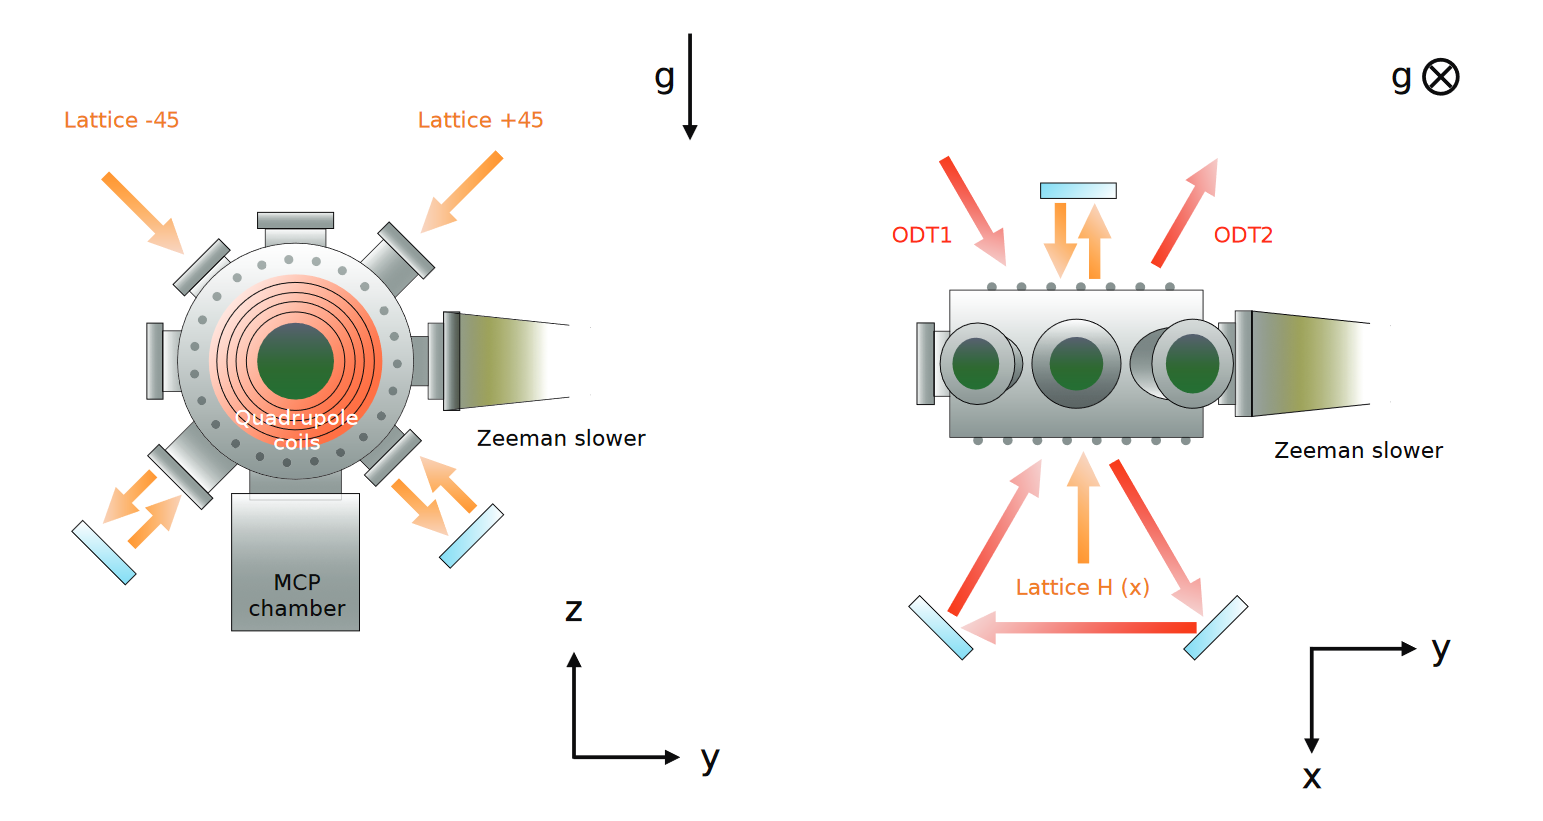
\includegraphics[width=\textwidth]{Fig/Chapter3/scheme_odt_lattice.png}
    \caption{Orientation of the ODT and lattice beams in the experiment. Taken from \cite{cayla_these}.}
    \label{fig:scheme_odt_lattice}
\end{figure}

\section{3D optical lattice}

\section{Electronic detection: The Micro Channel Plate Detector}

\section{Two-photon Raman transfer}

As we have seen in the first sections of this chapter, the BEC is prepared in the magnetic-substate $m_j=1$. To make a proper measurement of the in-trap momentum of the atoms, it is absolutely crucial that their TOF trajectories are not perturbed, notably by interactions with magnetic fields. Indeed, it would be quite hard to shield the science chamber from every unwanted magnetic field on the large distance of $\sim 50 \ \rm{cm}$ on which we let the atoms fall. A solution to cancel these unwanted interactions is to transfer the atoms into the non-magnetic sub-state $m_j=0$. All non-transferred atoms are then removed by applying a strong magnetic gradient.

When I started my PhD, the preferred method was to use a magnetic field bias to separate the different sub-states with the Zeeman effect and then drive the transition between $m_j=1$ and $m_j=0$ with a RF wave. However, the energy difference between the sub-states $m_j=1$ and $m_j=0$ and $m_j=0$ and $m_j=-1$ is the same. We therefore rather have a 3-level system with two resonant transitions and can only achieve a $50\%$ population transfer to $m_j=0$. This has a strong consequence: only half of the atoms reach the BEC, thus reducing the detection efficiency by a factor 2. This is particularly harmful for two-body correlation measurements such as \kmk pairing as we need to detect the two atoms of the pair: losing a factor on the detection efficiency reduces the probability to detect a \kmk pair by a factor $2^2=4$. This calls to change the transfer scheme to achieve a $100\%$ (or close to) population transfer to the $m_j=0$ state.

To do so, we will rather use an optical transfer scheme, the two-photon Raman transfer. While this was used on our experiment a few years back on the $2 \ ^3 S_1 \rightarrow 2 \ ^3 P_1$, it was abandoned as spontaneous emission effects were perturbing the measured momentum distribution to sufficiently high levels, harming the measurements conducted at the time. Our goal to detect \kmk pairs, as well as the recent addition of a third laser source allowing us to address the remaining transition $2 \ ^3 S_1 \rightarrow 2 \ ^3 P_0$ better suited for two-photon Raman transfer (\NOTE{WHY?}) motivated us to build the required setup. In this section, we will explain the theory behind the two-photon Raman transfer before presenting the experimental setup and the procedure to characterize it.

\subsection{Principle of the two-photon Raman transfer}

% Raman scattering is an inelastic scattering process of a photon by an atom resulting in a modification of the internal state of the atom. 

To understand what two-photon Raman transfer is, let us consider a lambda level structure with two ground states $\ket{g_1}$,$\ket{g_2}$ and one excited state $\ket{e}$ (see Fig.-\ref{fig:raman_level}). Raman scattering is an inelastic process in which the atom absorbs a first photon of frequency $\omega_1$ and re-emits a photon of frequency $\omega_2$, changing its internal state from $\ket{g_1}$ to $\ket{g_2}$. The absorbed photon is called the \textbf{pump} photon and the emitted one the \textbf{Stokes} photon. The energy difference between the absorbed and scattered photons corresponds to the energy difference $\Delta E$ between the two states $\ket{g_1}$ to $\ket{g_2}$. If the modes $\omega_1$ and $\omega_2$ are populated, for instance if we shine laser light on the atom at these two frequencies, the process can be stimulated as the probability to emit a photon in a given mode is more likely the more photons there are in the mode. It is therefore possible exploit this effect to realize a population transfer from the state $\ket{g_1}$ to the state $\ket{g_2}$.

% If the two lasers are not copropagating, this method can be used to to transfer momentum to the atoms and change their trajectory. As this is not something we want to do, we use to copropagating laser beams.

\begin{figure}
    \centering
    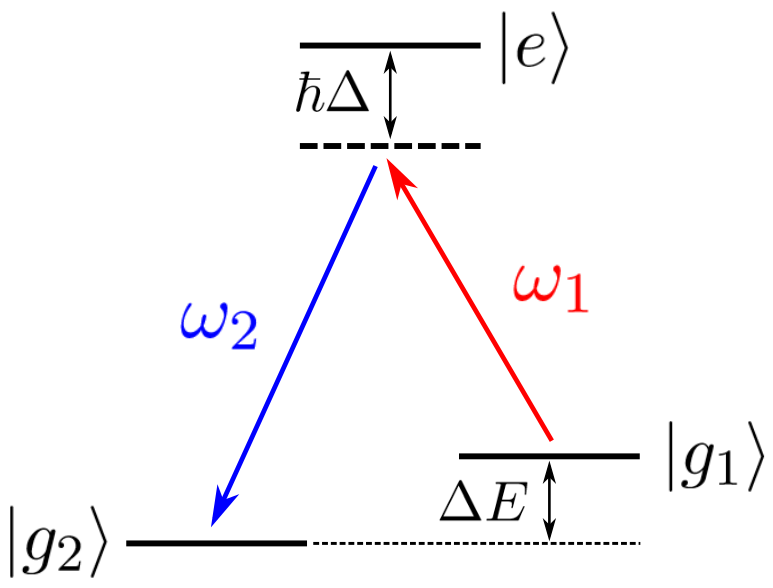
\includegraphics[width=0.5\textwidth]{Fig/Chapter3/raman_level.png}
    \caption{Caption}
    \label{fig:raman_level}
\end{figure}


Importantly, the detuning $\Delta=(\omega_{e}-\omega_{g_1})-\omega_1=(\omega_{e}-\omega_{g_2})-\omega_2$ (see Fig.-\ref{fig:raman_level}) must be large to avoid one photon absorption, {\it i.e.} population of the excited state and spontaneous emission. In these conditions, the excited level can be adiabatically eliminated to describe the two-photon transfer as an effective two-level coupling between $\ket{g_1}$ and $\ket{g_2}$. The system then undergoes well-known Rabi oscillations of frequency:

\begin{equation}
    \Omega_{\rm{eff}}= \sqrt{\frac{\Omega_1^2 \Omega_2^2}{4 \Delta^2} + \delta_{\rm{2p}}^2}
\end{equation}

\noindent where $\Omega_1$ and $\Omega_2$ are the Rabi frequencies associated to laser fields 1 and 2 and $\delta_{\rm{2p}}$ is the detuning to the two-photon resonance condition $\delta_{\rm{2p}}=(\omega_{g_2} - \omega_{g_1}) - (\omega_2-\omega_1)$. The maximum transfer efficiency is the ratio $\eta_{\rm{2p}}=\Omega_{\rm{2p}}^2 /\Omega^2_{\rm{eff}}$ where $\Omega_{\rm{2p}}=\frac{\Omega_1 \Omega_2}{2 \Delta}$ is the effective two-photon Rabi frequency. For $\delta_{\rm{2p}}=0$, we get $\eta_{\rm{2p}}=1$ meaning that it is possible to transfer the entire population of $\ket{g_1}$ to $\ket{g_2}$.

\subsection{Experimental implementation}

To implement the two-photon Raman transfer, we use the transition $2 \ ^3 S_1 \rightarrow 2 \ ^3 P_0$ that effectively realize the lambda structure required for Raman transfer (see Fig.-\ref{fig:raman_He}). The pump beam is $\sigma_-$ polarized and the Stokes beam $\pi$ polarized. We opt for a configuration with co-propagating beams to keep the trajectory of the atoms the same.



\begin{figure}
    \centering
    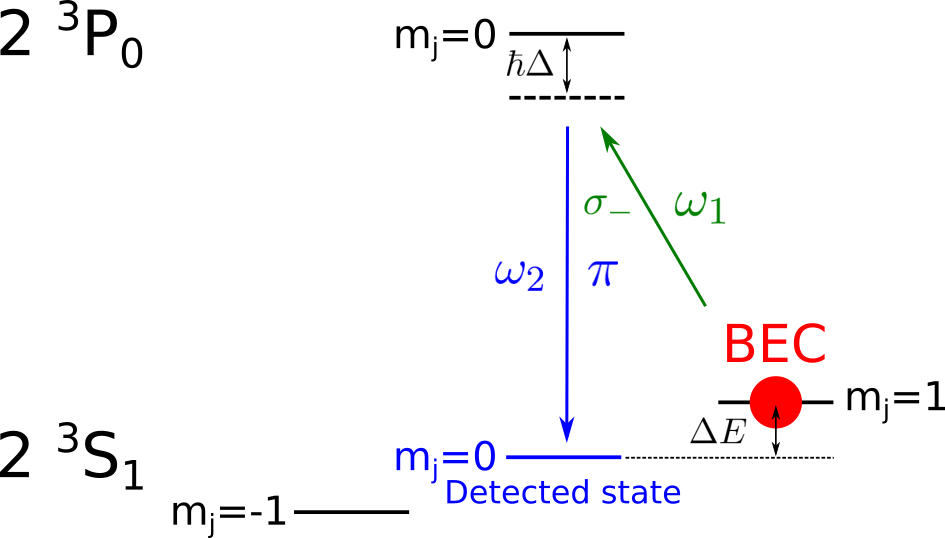
\includegraphics[width=0.7\textwidth]{Fig/Chapter3/raman_exp.png}
    \caption{Implementation of the two-photon Raman transfer with $^4 \rm{He}^*$.}
    \label{fig:raman_He}
\end{figure}

The optical setup is represented in Fig.-\ref{fig:raman_table}. In brief, the two beams are obtained from a single homemade External-Cavity Diode Laser, locked on the $2 \ ^3 S_1 \rightarrow 2 \ ^3 P_0$ of frequency $\nu_0$ via saturated absorption spectroscopy. Actually, in the saturated absorption spectroscopy arm of the setup, the frequency of the laser is shifted by $400 \ \rm{MHz}$ by a double pass Acousto-Optic Modulator (AOM) before locking (see Fig.-\ref{fig:raman_table}, meaning that the frequency of the laser is $\nu = \nu_0 - 400 \ \rm{MHz}$. The main beam is then split in two beams whose respective power are controlled by rotating a half-wave plate in front of a polarizing beam-splitter cube. The frequencies of each beam is set by another double pass AOM. In the end, the frequencies are $\nu_{\rm{Stokes}} = \nu_0 - 800 \ \rm{MHz}$ for the Stokes beam and $\nu_{\rm{Pump}} = \nu_0 - 813 \ \rm{MHz}$ for the pump beam. The small difference of $13 \ \rm{MHz}$ is set to match the energy difference $\Delta E$ between the sub-states $m_j=0$ and $m_j=1$ that we control by applying a magnetic bias field along the $x$ direction. The detuning to the one-photon transition is $|\Delta|=800 \ \rm{MHz}$ which is large enough to avoid spontaneous emission effects. The polarizations of the two beams are set to be linear and orthogonal. They are finally sent on two faces of a polarizing beam-splitter cube to be overlapped and coupled into a polarization-maintaining fiber bringing them to the science chamber as illustrated on Fig.-\ref{fig:raman_sc}.

\begin{figure}
    \centering
    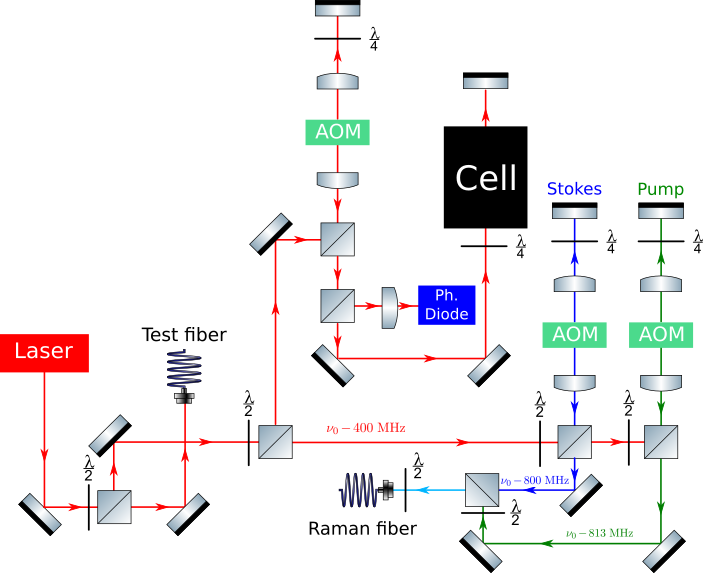
\includegraphics[width=\textwidth]{Fig/Chapter3/table_raman.png}
    \caption{Optical setup for two-photon Raman transfer. After being frequency locked via saturated absorption spectroscopy, the laser beam is split to produce the Stokes and pump beam. The powers are controlled with half-wave plates and polarizing beam splitter, while the frequencies are controlled with Acousto-Optic Modulators.}
    \label{fig:raman_table}
\end{figure}

The polarization at the exit of the fiber is set by a half-wave plate so that the Stokes beam is linearly polarized along the quantification axis $x$ to have the $\pi$ polarisation. The pump beam is linearly polarized as well but orthogonal to the Stokes beam polarisation. This decomposes as the sum of a $\sigma_+$ and $\sigma_-$ polarisation for the atoms. Because of the energy levels structure, the $\sigma_+$ component does not interact with the atom, leaving only the effect of the wanted $\sigma_-$ polarization. This means however than half of the power of the pump beam is useless, we thus need to put twice more power for the pump beam than for the Stokes beam for a symmetric configuration.


\begin{figure}
    \centering
    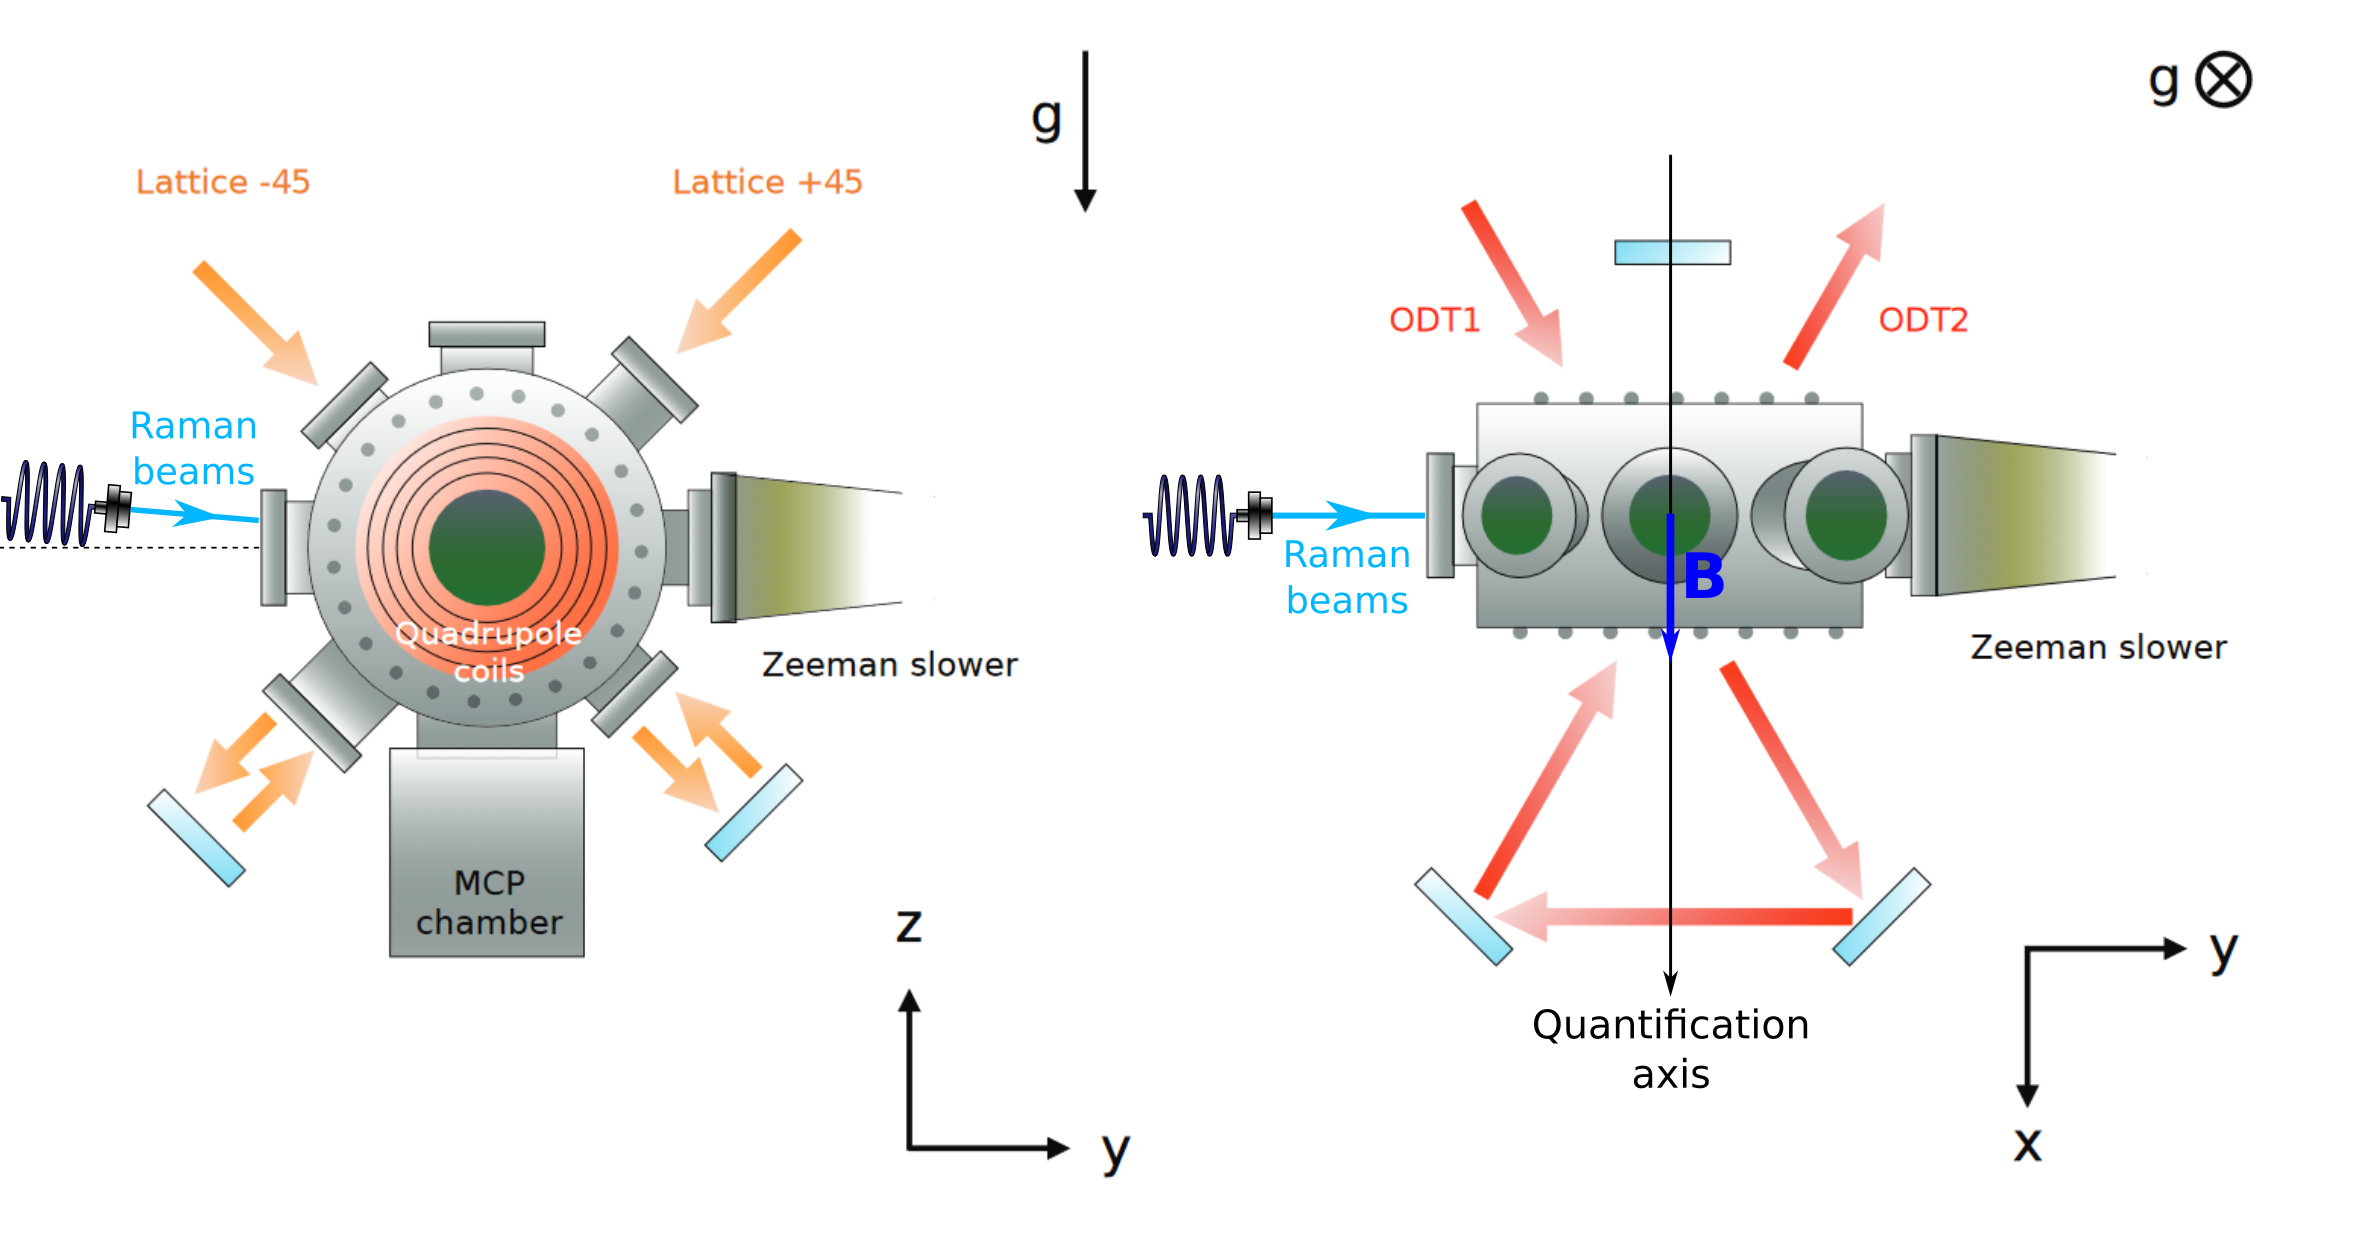
\includegraphics[width=\textwidth]{Fig/Chapter3/raman_sc.png}
    \caption{Orientation of the Raman beams in the experiment. On the right picture, the blue arrow denotes the orientation of the magnetic bias field, setting the quantification axis.}
    \label{fig:raman_sc}
\end{figure}

\subsection{Measurement of the two-photon resonance}

As previously discussed, the transfer efficiency is highly dependent from the detuning to the two-photon resonance condition set by the frequency difference $\Delta \nu = \nu_{\rm{Stokes}} - \nu_{\rm{Pump}}$. It is therefore important to scan $\Delta \nu$ prior to any use of two-photon Raman transfer to set it perfectly on resonance. The procedure is the following:

\begin{itemize}
    \item We significantly reduce the power of the Raman beams ($30 \ \mu \rm{W}$ and $60 \ \mu \rm{W}$ before the fiber for the Stokes and pump beams respectively) to avoid power broadening of the transition and to have a small Rabi frequency. The period of the Rabi oscillations is then large, we can therefore use a pulse long enough to obtain the necessary frequency resolution, but short enough so that we remain in the first Rabi oscillation when the detuning changes. We chose a pulse duration of $60 \ \mu \rm{s}$. \NOTE{T RABI IN COMPARISON}
    \item We prepare a Mott insulator whose large momentum distribution prevents saturation effects of the detector from happening.
    \item We perform two-photon Raman transfer for different values of $\Delta \nu$ and plot the number of detected atoms by the MCP as a function of $\Delta \nu$. We finally fit the data to find the position of the resonance. 
\end{itemize}

\NOTE{ALLER CHERCHER LES DONNES D'UNE RESONANCE.}

\subsection{Rabi oscillations}

In order to check that the two-photon Raman transfer is working as intended, we measure Rabi oscillations for different power values and check that the Rabi frequency indeed scales linearly with power. Like when we measure the two-photon resonance, we perform the measurement on a Mott insulator to avoid saturation.

\NOTE{DONNEES RABI FLOPING}



\section{Characterisation of two-body collisions in the time-of-flight dynamics}

\subsection{Classical model}

\subsection{Evolution with total atom number}

\subsection{Evolution with lattice depth}

\subsection{Conclusion}

\section{Adiabatic preparation in the vicinity of the Mott transition}

\subsection{Thermometry method}

\subsection{Fischer information and Cramér-Rao bound}

\subsection{Entropy measurement}
